\section{Plano Operacional}

\subsection{Layout físico}

O escritório da empresa seguiria, inicialmente, seguiria o seguinte
modelo:

\begin{figure}[H]
\centering
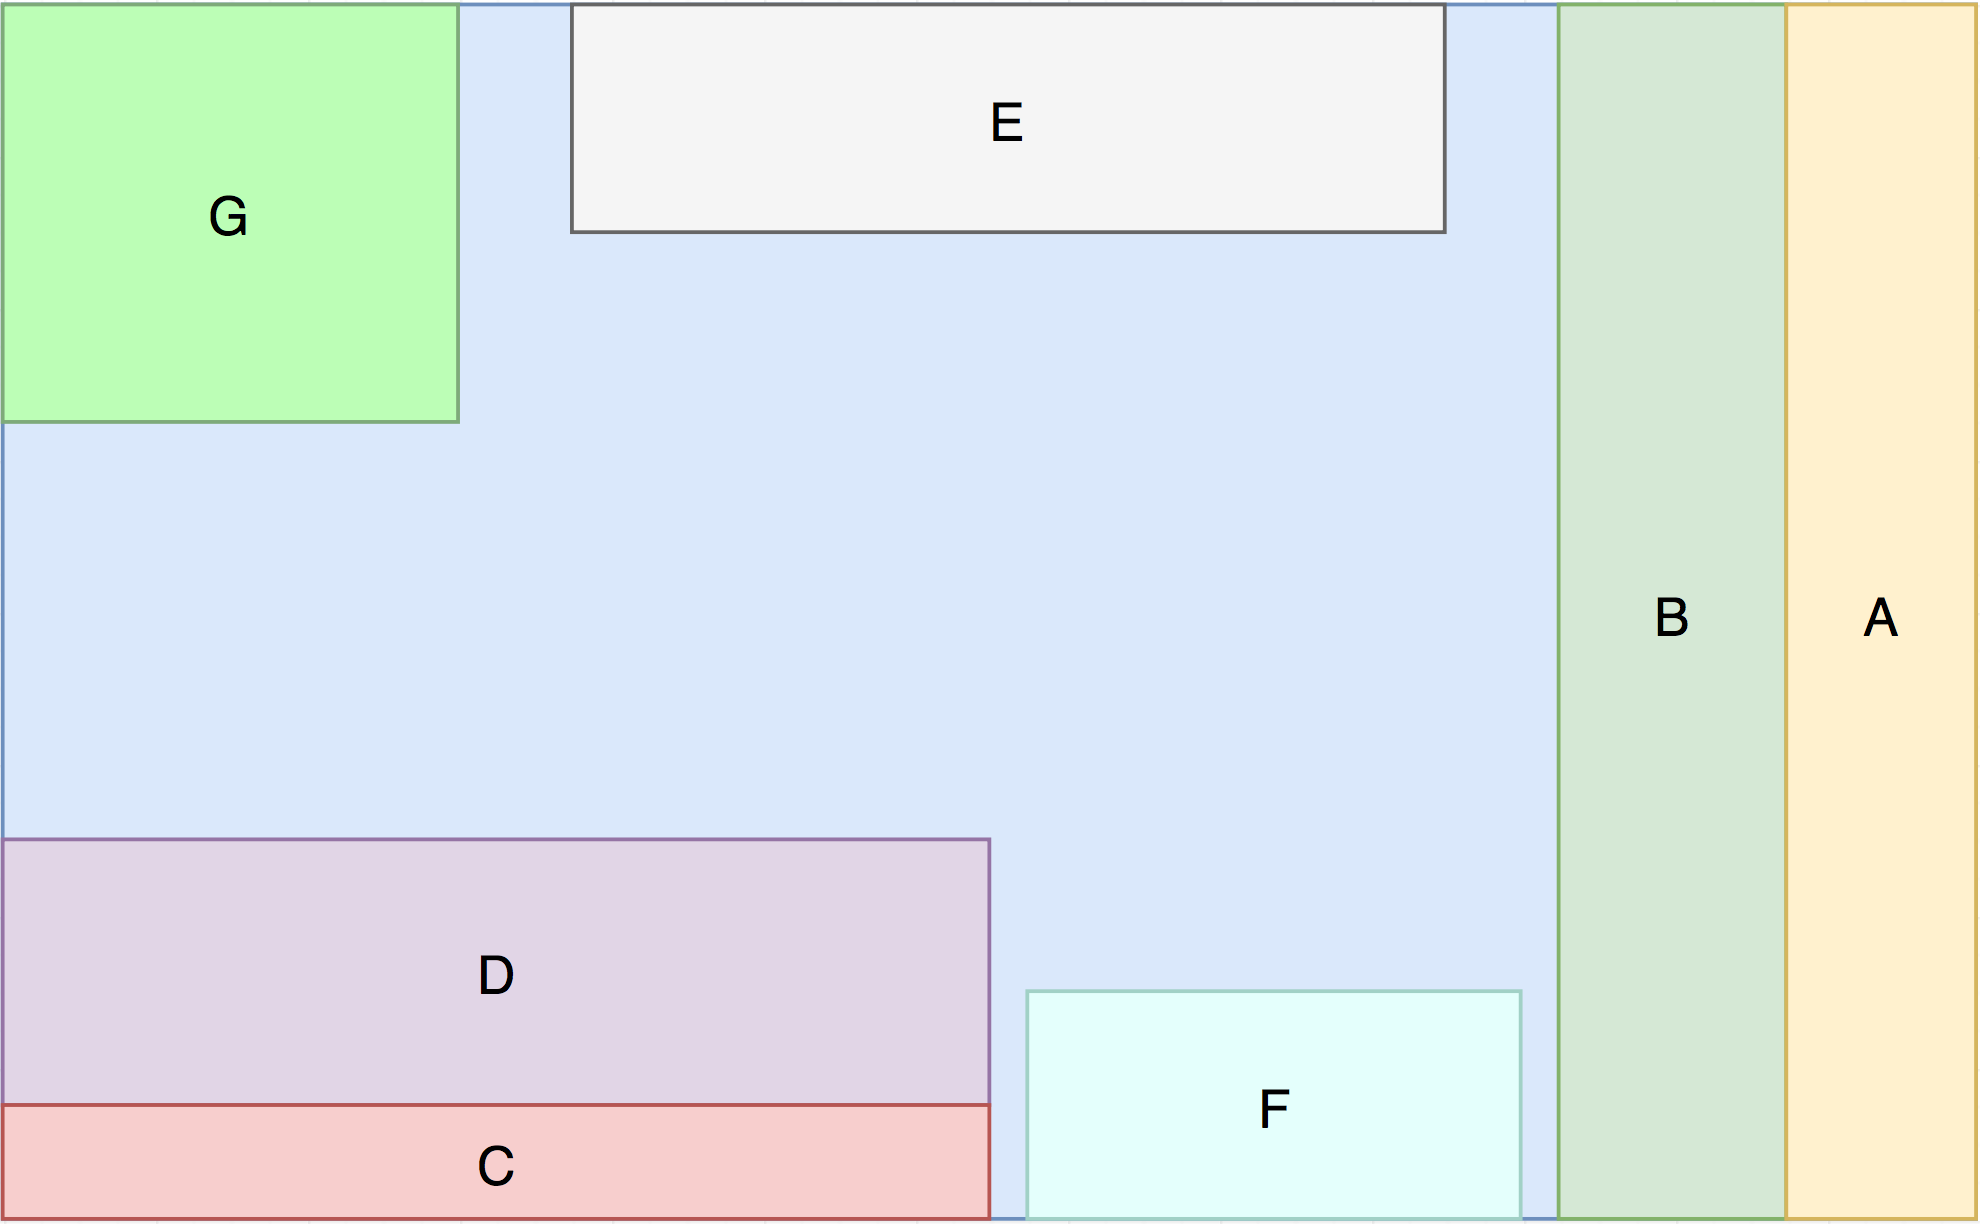
\includegraphics[width=4.875in]{layoutfisico.png}
\caption{Layout físico do escritório da empresa.}
\label{fig:layoutfisico}
\end{figure}

Onde o espaço (de aproximadamente $7$ x $5$ $m^2$) está dividido
da seguinte forma:

\begin{itemize}
	\item A: Armários elevados e prateleiras para armazenamento de 
	componentes e de \emph{Drones} montados.
	\item B: Bancada de manutenção, montagem e testes. Contém ao 
	menos um computador, um osciloscópio, aparelho de soldagem, 
	fonte de alimentação, multímetros, conjuntos de chaves de 
	parafusos etc.
	\item C: Quadro branco e prateleira de livros para consulta.
	\item D: Bancada com ao menos dois computadores para projeto,
	desenvolvimento e simulações.
	\item E: Setor administrativo. Escrivaninha com um computador
	para gerenciar pedidos, contato com clientes, finanças e 
	compras.
	\item F: Copa. Bancada com pia, armários elevados, caferira,
	frigobar e microondas.
	\item G: Sanitário.
\end{itemize}

Vale ressaltar que esse layout certamente será modificado com 
o crescimento da empresa. Como, inicialmente, serão necessárias
poucas pessoas, conclui-se que uma organização desse tipo seria
suficiente para manter o desenvolvimento e customização do 
controlador dadas as demandas.

Além disso, a produção do controlador de voo comercial se dará 
externamente, ficando os setores $A$ e $B$ dedicados apenas a 
testes e à montagem e manutenção das aeronaves que serão utilizadas 
em prestação de serviços pela própria empresa.

\subsection{Layout operacional}

O layout operacional trata da divisão de tarefas de forma 
hierárquica dentro da empresa e seguirá, inicialmente, o seguinte
modelo:

\begin{figure}[H]
\centering
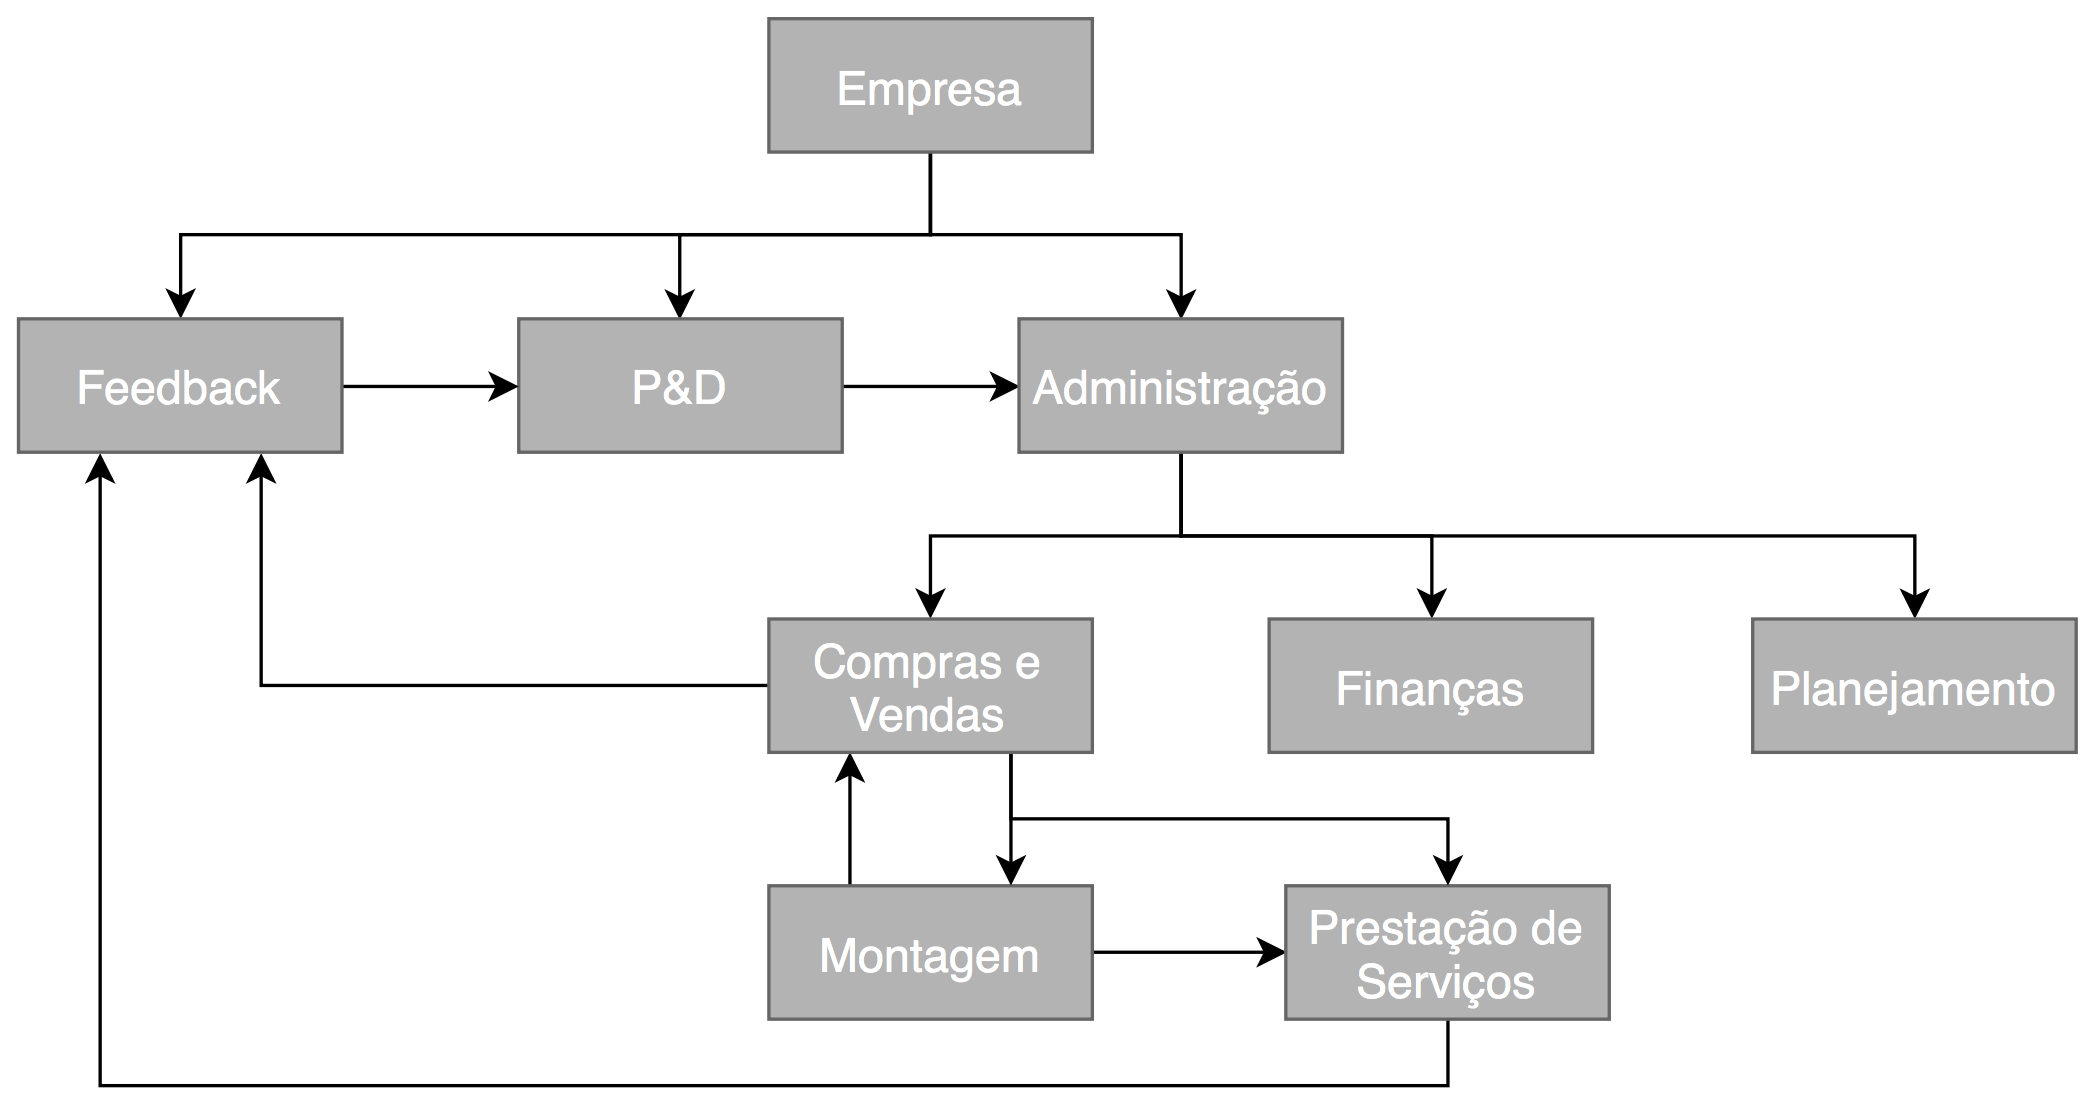
\includegraphics[width=\textwidth]{layoutoperacional.png}
\caption{Layout operacional da empresa.}
\label{fig:layoutoperacional}
\end{figure}

Enfatiza-se a importância do setor "Feedback": como a empresa
é nova no mercado, é importante levar em consideração os 
fatores externos e principalmente a opinião do cliente quanto 
à qualidade dos produtos e serviços ofertados. Para tanto,
planeja-se, baseando-se em \cite{leanstartup}, realizar 
ciclos rápidos de desenvolvimento e aprendizado, de forma
a evitar desperdícios de tempo e recursos trabalhando em algo
que não atende as demandas dos clientes (e, consequentemente,
dando vantagem à concorrência). O setor "Feedback"\ será
o principal "termômetro"\ do setor de Pesquisa \& 
Desenvolvimento, orientando o foco produtivo da empresa.

\subsection{Capacidade produtiva}

Uma vez que a empresa tenha uma versão comercial do \emph{
firmware} do controlador de voo, junto a um projeto do seu
circuito, a capacidade produtiva de controladores de voo 
estará limitada pelo investimento inicial, o qual permitirá
os primeiros pedidos das primeiras unidades a serem vendidas.

Algumas das unidades pedidas serão retidas na empresa e 
utilizadas para montar uma frota de cerca de 4 \emph{Drones}
os quais serão utilizados nos primeiros projetos de prestação
de serviço. Estes serão limitados pela capacidade de
deslocamento da equipe (principalmente para áreas agrícolas,
onde a prestação de serviço é prioritária por ter maior
potencial de retorno).

A longo prazo, almeja-se aumentar a capacidade produtiva de
controladores conforme aumentar o capital de giro da empresa,
também através de prestações de serviço. A capacidade de 
prestações também será aumentada conforme a empresa contratar
empregados que permitirão maior \emph{throughput} em 
atendimento a clientes.

\subsection{Processos Operacionais}



\subsection{Necessidade de pessoal}


